\documentclass{article}

\usepackage{fancyhdr}
\usepackage{extramarks}
\usepackage{amsmath,amssymb,mathrsfs}
\usepackage{amsthm}
\usepackage{amsfonts}
\usepackage{parskip}
\usepackage[version=3]{mhchem} 
\usepackage{fixltx2e}
\usepackage{refcount}
\usepackage{siunitx}
\usepackage{lastpage}
\usepackage{textcomp}
\usepackage{xfrac}
\usepackage{lmodern}
\usepackage{cool}
\usepackage{cancel}
\usepackage{microtype}
\usepackage{gensymb}
\usepackage{enumerate}
\usepackage{float}
\usepackage{bm}
\usepackage{csquotes}
\usepackage{mathtools}
\usepackage{mcode}

\usepackage[hidelinks]{hyperref}

\DeclarePairedDelimiter\bra{\langle}{\rvert}
\DeclarePairedDelimiter\ket{\lvert}{\rangle}
\DeclarePairedDelimiterX\braket[2]{\langle}{\rangle}{#1 \delimsize\vert #2}








%
% Basic Document Settings
%

\topmargin=-0.45in
\evensidemargin=0in
\oddsidemargin=0in
\textwidth=6.5in
\textheight=9.0in
\headsep=0.25in

\linespread{1.1}

\clubpenalty = 10000
\widowpenalty = 10000

\pagestyle{fancy}
\lhead{\hmwkAuthorName}
\chead{\hmwkClass\ \textemdash\ \hmwkTitle}
\rhead{\firstxmark}
\lfoot{\lastxmark}
\cfoot{ASV\twodigits{\thepage}\ of \twodigits{\getpagerefnumber{LastPage}}}

\renewcommand\headrulewidth{0.4pt}
\renewcommand\footrulewidth{0.4pt}

\setlength\parindent{0pt}
\setlength\parskip{1.2ex}





%
% Create Problem Sections
%

\newcommand{\enterProblemHeader}[1]{
    \nobreak\extramarks{}{Problem \arabic{#1} continued on next 
page\ldots}\nobreak{}
    \nobreak\extramarks{Problem \arabic{#1} (continued)}{Problem \arabic{#1} 
continued on next page\ldots}\nobreak{}
}

\newcommand{\exitProblemHeader}[1]{
    \nobreak\extramarks{Problem \arabic{#1} (continued)}{Problem \arabic{#1} 
continued on next page\ldots}\nobreak{}
    \stepcounter{#1}
    \nobreak\extramarks{Problem \arabic{#1}}{}\nobreak{}
    
}

\setcounter{secnumdepth}{0}
\newcounter{partCounter}
\newcounter{homeworkProblemCounter}
\setcounter{homeworkProblemCounter}{1}
\nobreak\extramarks{Problem \arabic{homeworkProblemCounter}}{}\nobreak{}

%
% Homework Problem Environment
%
% This environment takes an optional argument. When given, it will adjust the
% problem counter. This is useful for when the problems given for your
% assignment aren't sequential. See the last 3 problems of this template for an
% example.
%
\newenvironment{homeworkProblem}[1][-1]{
    \ifnum#1>0
	\setcounter{homeworkProblemCounter}{#1}
    \fi
%     \section{Problem \arabic{homeworkProblemCounter}}
    \setcounter{partCounter}{1}
    \enterProblemHeader{homeworkProblemCounter}
}{
    \exitProblemHeader{homeworkProblemCounter}
    \pagebreak

}

%
% Homework Details
%   - Title
%   - Due date
%   - Class
%   - Instructor
%   - Author
%

\newcommand{\hmwkTitle}{Homework\ \# 02}
\newcommand{\hmwkDueDate}{04 October 2016}
\newcommand{\hmwkClass}{NE 255}
\newcommand{\hmwkClassInstructor}{Professor Rachel Slaybaugh}
\newcommand{\hmwkAuthorName}{Andrew S Voyles}

%
% Title Page
%

\title{
%     \vspace{2in}
    \textmd{\textbf{\hmwkClass:\ \hmwkTitle}}\\
    \normalsize\vspace{0.1in}\small{Due\ \hmwkDueDate}\\
    \vspace{0.1in}\large{\textit{\hmwkClassInstructor}}
}

\author{\textbf{\hmwkAuthorName}}
\date{}

\renewcommand{\part}[1]{\textbf{\large Part 
\Alph{partCounter}}\stepcounter{partCounter}\\}

%
% Various Helper Commands
%

% Useful for algorithms
\newcommand{\alg}[1]{\textsc{\bfseries \footnotesize #1}}

% For derivatives
\newcommand{\deriv}[1]{\frac{\mathrm{d}}{\mathrm{d}x} (#1)}

% For partial derivatives
\newcommand{\simplepderiv}[2]{\frac{\partial}{\partial #1} (#2)}

% Integral dx
\newcommand{\dx}{\mathrm{d}x}

% Alias for the Solution section header
\newcommand{\solution}{\textbf{\large Solution}}

% One sentence of lorem ipsum text
\newcommand{\shortlipsum}{Lorem ipsum dolor sit amet, consectetuer adipiscing 
elit.}

% Pad zeroes for footer numbering
\newcommand\twodigits[1]{%
  \ifnum#1<10 0#1\else #1\fi
}

% Consistant figure references
\newcommand{\figref}[1]{Figure~\ref{#1}}

% Define partial derivative alias
\newcommand{\partialder}[2]{\dfrac{\partial #1}{\partial #2}}

% Volume symbol
\newcommand{\volume}{\mathop{\ooalign{\hfil$V$\hfil\cr\kern0.08em--\hfil\cr}}\nolimits}

% Area symbol
\newcommand{\area}{\mathop{\ooalign{\hfil$A$\hfil\cr\kern0.08em--\hfil\cr}}\nolimits}

% Sin and Cos with auto-parentheses 
\newcommand{\sinp}[1]{\sin{\left( #1\right)}}
\newcommand{\cosp}[1]{\cos{\left( #1\right)}}
\newcommand{\expp}[1]{\exp{\left( #1\right)}}
\newcommand{\sinhp}[1]{\sinh{\left( #1\right)}}
\newcommand{\lnp}[1]{\ln{\left( #1\right)}}
\newcommand{\pp}[1]{\left( #1\right)}
\newcommand{\sci}[2]{ #1 \cdot 10^{#2}\ }
\newcommand{\angstrom}{\mbox{\normalfont\AA}}
\newcommand{\norm}[1]{\lVert #1 \rVert}






% math syntax
\newcommand{\nth}{n\ensuremath{^{\text{th}}} }
\newcommand{\ve}[1]{\ensuremath{\mathbf{#1}}}
\newcommand{\Macro}{\ensuremath{\Sigma}}
\newcommand{\rvec}{\ensuremath{\vec{r}}}
\newcommand{\xvec}{\ensuremath{\vec{x}}}
\newcommand{\omvec}{\ensuremath{\hat{\Omega}}}
\newcommand{\vOmega}{\ensuremath{\hat{\Omega}}}


% Make vectors use boldface
\renewcommand{\vec}[1]{\mathbf{#1}}


% Consistant matrix notation
\newcommand{\matr}[1]{\mathbf{#1}} % undergraduate algebra version
% \newcommand{\matr}[1]{#1}          % pure math version
% \newcommand{\matr}[1]{\boldsymbol{#1}}     % ISO complying version


\makeatletter
% Make common definition of mean
\newcommand*\mean[1]{\overline{#1\raisebox{3mm}{}}}

\makeatother






\begin{document}

\maketitle
\thispagestyle{fancy}





\section{Problem 1}

\begin{homeworkProblem}


 Determine the macroscopic scattering cross section of UO\(_2\) as a function of
a generic enrichment factor \(\gamma = N_{U-235}/N_{U-238}\) where \(N\) is the atom density. Find
its value assuming a density of 10 g/cm\(^3\), \(\sigma^U_s \backsimeq\) 8.9 b and \(\sigma^O_s \backsimeq\)  3.75 b, and 5\% weight enrichment.




\subsection{Solution}
    
   The macroscopic cross section for a compound is defined in terms of its constituent atoms:
   
   \begin{equation}
\Sigma_s^{UO_2} = N_U\sigma_s^U + N_O\sigma_s^O
\end{equation}

As described, we will define a generic enrichment factor, \(\gamma\), in terms of both atom density \(N_i\) and isotopic atom fractions \(\alpha_i\): 

\begin{equation}
\begin{split}
\gamma &= \dfrac{N_{U-235}}{N_{U-238}}
\\
&= \dfrac{\alpha_{U-235}N_{UO_2}}{\pp{1-\alpha_{U-235}} N_{UO_2}}
\\
&= \dfrac{\alpha_{U-235}}{1-\alpha_{U-235}} 
\end{split}
\end{equation}

Inverting this, we can calculate \(\gamma\) in terms of \(\alpha_{U-235}\), which will useful for later on:

\begin{equation}
\alpha_{U-235} = \dfrac{\gamma}{\gamma+1}
\end{equation}

The molar mass of UO\(_2\) (in g/mol) can be thus calculated in terms of the atomic enrichment in U-235:

\begin{equation}
\begin{split}
M_{UO_2} &= M_U + 2M_O
\\
&= \alpha_{U-235}M_{U-235} + \pp{1-\alpha_{U-235}} M_{U-238} + 2M_O
\\
&= \dfrac{\gamma}{\gamma+1} M_{U-235} + \dfrac{1}{\gamma+1} M_{U-238} + 2M_O
\\
&= \dfrac{\gamma}{\gamma+1} \pp{235} + \dfrac{1}{\gamma+1} \pp{238} + 32
\end{split}
\end{equation}

The number density of  UO\(_2\) (in atoms/cm\(^3\)) is thus simply:

\begin{equation}
\begin{split}
N_{UO_2} &= \dfrac{\rho_{UO_2} N_A}{M_{UO_2}}
\\
&= \dfrac{\rho_{UO_2} N_A}{\dfrac{\gamma}{\gamma+1} \pp{235} + \dfrac{1}{\gamma+1} \pp{238} + 32}
\\
&= \rho_{UO_2} N_A \dfrac{\gamma+1}{3\pp{89\gamma+90}}
\end{split}
\end{equation}

By stoichiometry, \(N_U = N_{UO_2}\) and \(N_O = 2N_{UO_2}\), making our final expression:

.\begin{equation}
\begin{split}
\Sigma_s^{UO_2} &= N_U\sigma_s^U + N_O\sigma_s^O
\\
&= \boxed{\rho_{UO_2} N_A \dfrac{\gamma+1}{3\pp{89\gamma+90}} \pp{\sigma_s^U + 2\sigma_s^O}} 
\end{split}
\end{equation} 

For a density of 10 g/cm\(^3\), \(\sigma^U_s \backsimeq\) 8.9 b and \(\sigma^O_s \backsimeq\)  3.75 b, and 5\% weight enrichment, we can calculate this macroscopic cross section:

\begin{equation}
\begin{split}
\alpha_{U-235} &= \dfrac{ \dfrac{\omega_{U-235}}{M_{U-235}} }{ \dfrac{\omega_{U-235}}{M_{U-235}} + \dfrac{1-\omega_{U-235}}{M_{U-238}} }
\\
&= \dfrac{ \dfrac{5\%}{235} }{ \dfrac{5\%}{235} + \dfrac{1-5\%}{238} }
\\
&= 5.061\%
\end{split}
\end{equation}

\begin{equation}
\begin{split}
\gamma &=\dfrac{\alpha_{U-235}}{1-\alpha_{U-235}} 
\\
&=\dfrac{5.061\%}{1-5.061\%} 
\\
&= 0.0533
\end{split}
\end{equation}

Thus,  

.\begin{equation}
\begin{split}
\Sigma_s^{UO_2} &= \rho_{UO_2} N_A \dfrac{\gamma+1}{3\pp{89\gamma+90}} \pp{\sigma_s^U + 2\sigma_s^O}
\\
&= \pp{10\ \sfrac{g}{cm^3}} \pp{\sci{6.022}{23}\sfrac{atoms}{mol}} \dfrac{0.0533+1}{3\pp{89\pp{0.0533}+90}\sfrac{g}{mol}} \pp{8.9 + 2\times3.75}10^{-24}\ cm^{2}
\\
&= \boxed{0.3659\ cm^{-1}}
\end{split}
\end{equation} 
    

\end{homeworkProblem}


\section{Problem 2}

\begin{homeworkProblem}

A major challenge in scientific computing is navigating the disparate architectures that
comprise new supercomputers.



\begin{enumerate}[(a)] 

\item  Look up the Top 10 supercomputing list and briefly describe the architecture
of the top three machines. List the number of machines of each type on the
top 10 (e.g. X are GPU-accelerated, Y contain MICs, etc.)





\subsection{Solution}
    
  According to the Top500 project\footnote{\url{https://www.top500.org/}}, the top three machines (ranked in terms of peak achieved floating-point-operations per second, FLOPS) are the Sunway TaihuLight, the TH-2, and Titan:
  
  The Sunway TaihuLight is at the \#1 spot on the Top500 list, and is a  93 PFLOP supercomputer in Wuxi, China, which first came online in June 2016. It uses 40,960 SW26010 processors clocked at 1.45 GHz, each of which contains 256 processing cores, for a total of 10,649,600 cores across the cluster. These are custom many-core processors using the RISC architecture, which eschews  typical cache structure for inter-core communication for a dedicated network between core clusters, which greatly improves the parallel efficiency of the cores. The machine is supported by 1.3 PBytes of RAM, and consumes approximately 15 MW of power. The machine runs on Sunway RaiseOS, a custom high-performance computing Linux distribution.  
  
  The Tianhe-2 is at the \#2 spot on the Top500 list, and is a  34 PFLOP supercomputer in Guangzhou, China, which first came online in June 2013. It uses 16,000 computing nodes, each of which contains two Intel Xeon E5-2692 12-core CPUs running at 2.2 GHz supported by 64 GB of RAM, and three Xeon Phi 31S1P co-processors, which contain 57 cores running at 1.1 GHz, supported by 8 GB of RAM. This is a combined 3,120,000 processing cores and 1.34 PBytes of RAM across the system, which consumes 17.6 MW of power.  The machine runs on Kylin, a custom high-performance computing Linux distribution.  
  
   Titan is at the \#3 spot on the Top500 list, and is a  17 PFLOP supercomputer Oak Ridge National Lab, in Oak Ridge, Tennessee, which first came online in October 2012. It uses 18,688 computing nodes, each of which contains one AMD Opteron 6274 16-core CPU running at 2.2 GHz supported by 32 GB of RAM, and one  Nvidia Tesla K20X GPU, which contains 2688 CUDA cores running at 732 MHz, supported by 6 GB of RAM. This is a combined 50,532,352 processing cores and 694 TBytes of RAM across the system, which consumes 8.2 MW of power.
   
   In this top 10 list, 6 computers (Sunway TaihuLight, Sequoia, Mira, Trinity, Hazel Hen, Shaheen II)  use massively multi-core custom primary CPUs as an architecture, 2 computers (Titan, Piz Daint) are GPU-accelerated,  1 computer (Tianhe-2 ) uses MICs / co-processors, and 1 computer (K-Computer) uses an alternative customs CPU architectures. 
 
   
\item   Describe the main characteristics of GPUs, MICs (multi integrated
cores), and CPUs-memory, clock speed, structure, etc.




\subsection{Solution}
    
   The CPU is the heart of a computer, the primary integrated circuit responsible for computation. The CPU receives instructions from some compiled binary code, decodes these instructions into a series of electrical commands, and then electrically connects its internal transistors, to perform the requested computation or operation.  CPUs have small memory buffers called \emph{caches}, which are responsible for holding commands, outputs, and memory addresses, as well as facilitating data I/O between the CPU and the motherboard, which have sizes on the order of a few MB in modern CPUs.
   
   The commands read and executed by a CPU are measured in \emph{clock cycles}, a unit of time used to regulate the operation of the CPU. Clock cycles can be used to measure the time required to complete the electrical operation involved in reading in binary instructions, decoding them, and executing the requested operation. Each operation consists of multiple instruction signals, so the more clock cycles that a CPU can execute per unit time, the more operations it is capable of performing per unit time. Clock speed, the number of clock cycles per second, is measured in Hz, and is a common measure of the internal processing speed of a CPU.
   
   A co-processor or multi-integrated core (MIC) is a sort of secondary processor, which is always paired with at least one primary CPU in a computing node. This design greatly accelerates computation by offloading intense and parallelizable sections of computation from the primary CPUs (which are optimized for several large serial tasks, due to their high clock speed) to the multiple cores in the co-processor, each of which are optimized for small, independent tasks, due to their lower clock speed. This allows a MIC to split a long serial computation into a very short parallel operation, assuming that the code is capable of being translated into an algorithm supporting parallel operation, such as finite element analysis.
   
   A GPU (graphical processing unit) is another type of processor, very similar in design to a MIC. Like a MIC, GPUs are processors comprised of hundreds to thousands of slower-clock speed cores, each of which has its own memory buffer. Traditionally, GPUs are used generate computer images and video, a process which is extremely demanding on the CPU. By moving these processes to a separate processor, the GPU, the CPU is freed up to focus on more intensive serial operations. Since the process of rendering these graphics is a naturally parallel task, the many small GPU cores turn a very CPU-intensive process into a much more trivial parallel task. To handle all of the data used during these parallel tasks, most modern GPUs have their own dedicated memory, on the order of several to tens of GB.
   
   \item Based on what we've talked about so far, postulate challenges of solving
the neutron transport equation in a way that would work on all of these architectures.



\subsection{Solution}
    
   We have discussed the two primary computational solution methods: deterministic methods, which discretize a large problem into multiple small elements, each of which is solved analytically. These problems are often hard to perform in parallel, but are well-suited to solution using many high-clock speed CPUs, and are easily executed on multi-core supercomputers. Due to the nature of matrix diagonalization, many of these finite-element methods are now being ported to parallel computation, however.
   
   Monte Carlo methods, on the other hand, use random sampling of events in a probability distribution to look at aggregate behavior of systems. In neutron transport, we can simulate the lifetime and interactions of a single neutron as it is transported through a volume. By performing this for many (\(\gg 10^8\)) neutrons, we can solve the NTE for neutron fluxes in various volumes by building up a statistically significant number of particle histories. Since each particle is transported independently, these Monte Carlo problems are very well-suited to parallel computation, and are frequently  performed on MIC and GPU-accelerated machines.


\end{enumerate}

\end{homeworkProblem}


\section{Problem 3}

\begin{homeworkProblem}

We often measure convergence by comparing one iteration to the previous
iteration (rather than the solution, since we presumably don't know what it is). Imagine
that you have software that gives the following solution vectors:

\begin{figure}[H]
 \centering
 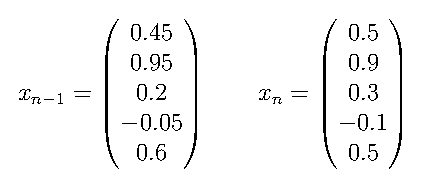
\includegraphics{./hw02_03a.pdf}
 % hw02_03a.pdf: 204x92 pixel, 72dpi, 7.20x3.25 cm, bb=0 0 204 92
\end{figure}


Calculate:




\begin{enumerate}[(a)] 

\item The absolute and relative error using the 1 norm.




\subsection{Solution}

For some vector \xvec, the \(\ell_1\) norm is calculated as:

\begin{equation}
 \norm{ \xvec }_1 = \sum_{i=1}^N \left| x_i \right|
\end{equation}

For some norm \(\norm{\cdot}\), we will define the absolute error between solution vectors \(x_n\) and \(x_{n-1}\) as:

\begin{equation}
\epsilon_A = \norm{x_n-x_{n-1}}
\end{equation}

Similarly, the relative error is:

\begin{equation}
\epsilon_R = \dfrac{ \norm{x_n-x_{n-1}}}{ \norm{x_n}} = \dfrac{ \epsilon_A}{ \norm{x_n}}
\end{equation}

Using these definitions and the  \(\ell_1\) norm:

\begin{equation}
\epsilon_A = \sum \pp{0.05, 0.05, 0.1, 0.05, 0.1  }^T = 0.35
\end{equation}

\begin{equation}
\epsilon_R = \dfrac{0.35}{ \sum \pp{0.5, 0.9, 0.3, 0.1, 0.5  }^T} = 0.1522
\end{equation}
 
   
\item   The absolute and relative error using the 2 norm




\subsection{Solution}

   
For some vector \xvec, the \(\ell_2\) norm is calculated as:

\begin{equation}
 \norm{ \xvec }_2 = \sqrt{\sum_{i=1}^N  x_i^2  }
\end{equation}
   
   
   
Using these definitions:

\begin{equation}
\epsilon_A = \sqrt{\sum \pp{0.0025, 0.0025, 0.01, 0.0025, 0.01 }^T} = 0.1658
\end{equation}

\begin{equation}
\epsilon_R = \dfrac{0.1658}{\sqrt{\sum \pp{0.25, 0.81, 0.09, 0.01, 0.25 }^T}} = 0.1397
\end{equation}
   
   
\item The absolute and relative error using the infinity norm.

What is most restrictive (that is, what would cause the code to converge first)?

Image that now \(x_{n-1} = (0.49, 0.92, 0.4, -0.09, 0.51)^T\). Recalculate the convergence values.

What do you observe? What does that mean about how you might select convergence
criteria?




\subsection{Solution}

  
For some vector \xvec, the \(\ell_\infty\) norm is calculated as:

\begin{equation}
 \norm{ \xvec }_\infty = \max_{1 \leq i \leq N} \left| x_i \right|
\end{equation}
   
   
   
Using these definitions:

\begin{equation}
\epsilon_A = \max \pp{0.05, 0.05, 0.1, 0.05, 0.1 }^T = 0.1
\end{equation}

\begin{equation}
\epsilon_R = \dfrac{0.1}{\max \pp{0.5, 0.9, 0.3, 0.1, 0.5  }^T} = 0.111
\end{equation}
   
   
\begin{table}[H]
\centering
\caption{Tabulated results for the various error criteria.}
\label{tab:firstx}
\begin{tabular}{c|c|c}
 Norm    & \(\epsilon_A\)     & \(\epsilon_R\)     \\ \hline
\(\ell_1\)   & 0.35   & 0.1522 \\
\(\ell_2\)   & 0.1658 & 0.1397 \\
\(\ell_\infty\) & 0.1    & 0.1111
\end{tabular}
\end{table}   

These results can be seen tabulated in \autoref{tab:firstx}. For most iterative methods, when the true solution is unknown, iteration continues until the error between two subsequent iterations falls below a set threshold. This leaves us with two ways to interpret convergence speed in the context of this problem. Since the \(\ell_\infty\) norm has the smallest of both the absolute and relative errors, it would predict that the two solution vectors are the closest to convergence, i.e., it would be the first to converge starting at the current timestep, assuming that the iterative method employed has monotonically decreasing errors between iterations. A second interpretation would be to look at the \(\ell_1\) norm, which has the largest of  both the absolute and relative errors. Many iterative solvers would see this as being \enquote{far} away from convergence, and take either a larger time step, or iterate more aggressively towards the solution, potentially reaching convergence first, at the risk of overshooting due to the \enquote{bang-bang} nature of aggressive iteration.

Repeating our analysis for the second \(x_{n-1}\) vector (with calculations not listed here for clarity, but verified in the \texttt{hw02\_03.m} script included in the parent repo), we see the results tabulated in \autoref{tab:firstx2}. Through inspection of these results, we that while the absolute errors have decreased in magnitude somewhat significantly from before, the relative errors have decreased by a smaller magnitude. Since the new \(x_{n-1}\) vector was closer to \(x_n\) than the old \(x_{n-1}\) vector, this illustrates why relative errors are typically used as convergence tolerances, as they normalize the scale of an error to its nominal value. 

It is also very important to point out that the \(\ell_\infty\) norms do not change at all for our new \(x_{n-1}\) vector. This is because , unlike the \(\ell_1\) and \(\ell_2\)  norms which look at the contributions of all errors between a pair of solution vectors, the \(\ell_\infty\)  only looks at the magnitude of the largest error contribution. While this can provide some stability against overshoot/undershoot by only focusing on minimizing the most significant error, it  ignores changes in the larger solution space, which can be used to give more feedback about one's proximity to convergence.

\begin{table}[H]
\centering
\caption{Tabulated results for the various error criteria, using the new \(x_{n-1}\).}
\label{tab:firstx2}
\begin{tabular}{c|c|c}
 Norm    & \(\epsilon_A\)     & \(\epsilon_R\)     \\ \hline
\(\ell_1\)   & 0.15   & 0.0652 \\
\(\ell_2\)   & 0.1034 & 0.0871 \\
\(\ell_\infty\) & 0.1    & 0.1111
\end{tabular}
\end{table}   
   

\end{enumerate}

\end{homeworkProblem}


\section{Problem 4}

\begin{homeworkProblem}

You have a piece of software that takes mesh spacing as an input variable.
Imagine that you have the following relative error values for each mesh spacing (\(h\)) /
number of mesh cells (N cells):

\begin{figure}[H]
 \centering
 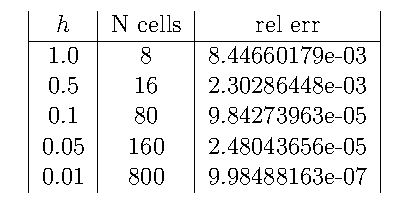
\includegraphics{./hw02_04a.pdf}
 % hw02_03a.pdf: 204x92 pixel, 72dpi, 7.20x3.25 cm, bb=0 0 204 92
\end{figure}



One of the ways we characterize method performance is the order of convergence. We'd
like to know how the error changes as we change the resolution of our discretization, in
this case, mesh spacing.

Using a log-log plot, plot relative error as a function of




\begin{enumerate}[(a)] 

\item  mesh spacing and






\subsection{Solution}
    
   Both plots shown here can be generated by running the \texttt{hw02\_04.m} script included in the parent repo.
   
   \begin{figure}[H]
 \centering
 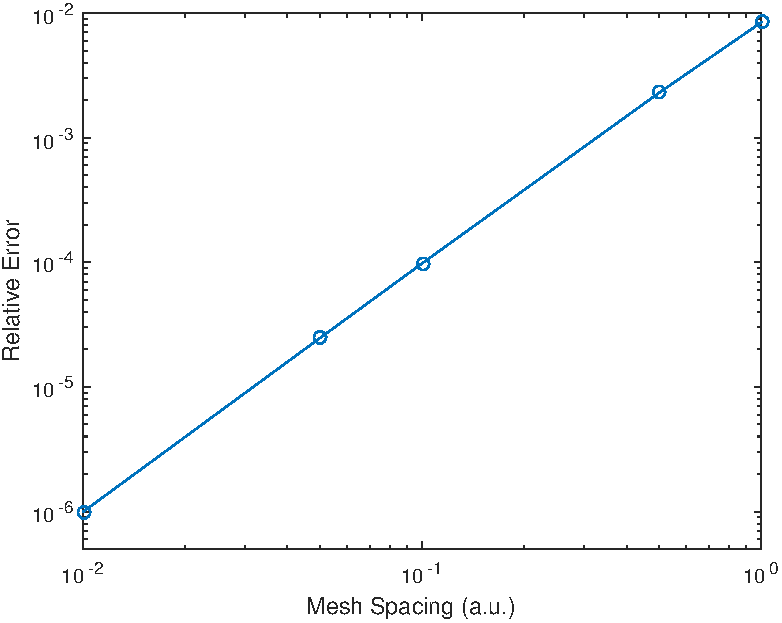
\includegraphics[scale=0.8]{./hw02_04a2.pdf}
 % hw02_04a.pdf: 199x105 pixel, 72dpi, 7.02x3.70 cm, bb=0 0 199 105
  \caption{Relative error as a function of mesh spacing.}
 \label{fig:problem4a}
\end{figure}



 
   
\item    cell count.

What is the functional relationship between error and mesh spacing / number of cells?




\subsection{Solution}
    
   
   \begin{figure}[H]
 \centering
 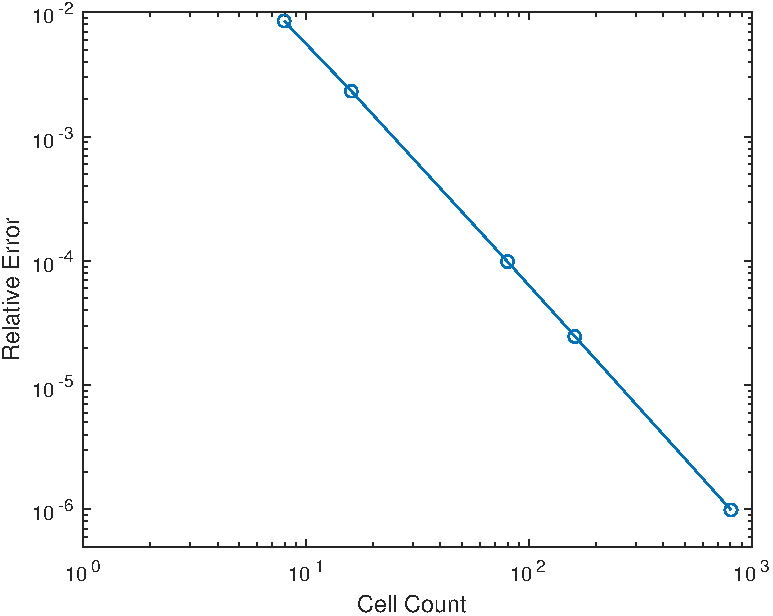
\includegraphics[scale=0.8]{./hw02_04b.pdf}
 % hw02_04a.pdf: 199x105 pixel, 72dpi, 7.02x3.70 cm, bb=0 0 199 105
 \caption{Relative error as a function of cell count.}
 \label{fig:problem4b}
\end{figure} 
 
We see in \autoref{fig:problem4a} that the points nearly perfectly across a line, whose slope was calculated as \(k = \dfrac{\Delta\pp{rel\ err}}{\Delta h} = 1.95\), which can be rounded to 2.0. Since this is in log-log space, the relative error, \(\epsilon_R\), can be concluded to be functionalized as \boxed{\epsilon_R \propto h^2.}

Similarly,  in \autoref{fig:problem4b} the points nearly perfectly across a line, whose slope was calculated as \(k = \dfrac{\Delta\epsilon_R}{\Delta N} = -1.95\), which can be rounded to -2.0. Since this is in log-log space, the relative error, \(\epsilon_R\), can be concluded to be functionalized as \boxed{\epsilon_R \propto \sfrac{1}{N^2}.}

\end{enumerate}

\end{homeworkProblem}


\section{Problem 5}

\begin{homeworkProblem}


What are six underlying assumptions in the neutron transport equation?
Write at least one sentence explaining what each assumption means and why we need
or want to make it.
  



\subsection{Solution}
    
  
\begin{enumerate}[(a)] 

\item All particles are zero-dimensional points, which behave classically, and ignoring quantum / fine structure effects. This means the the effective de Broglie wavelength of transport particles (primarily neutrons) is far smaller than the atomic length scale of the materials they are being transported through. This allows us to neglect quantum effects, and generalize the system, although later perturbations may be introduced, namely through cross sections. 

 
   
\item  Neutrons travel in straight paths in between interaction vertices. This saves the need to parameterize the transport and statistical nature of particle transport even further. By choosing a suitable coordinate system, and properly discretizing the system, particle transport can be achieved with acceptable resolution.


\item Neglect neutron-neutron interactions. All transported particles are independent. This linearizes the NTE, and allows for parallel calculations of the each transported particle.

\item The system volume is time-independent, i.e., \(\dfrac{dV}{dt} = 0\). Since the NTE is fundamentally accounting the neutrons in some control volume, this simplifies the transport, as a time-dependent volume would be 1) far harder to model in the first place, and 2) require changing boundary conditions, which are difficult to determine \emph{a priori} as a function of time.

\item The boundary of the control volume is a non-reentrant surface, that is, any neutrons which exit the control volume do not reenter at another point. This saves the trouble of tracking neutrons outside our control volume, which we typically define as slightly larger than the area of interest for a problem.

\item Material properties are isotropic, time-independent, and do not have significant deviations about an expected value. These prevent us from needing to do material properties at an atomic-scale resolution, but instead use bulk properties representative of the material. In addition, over the length of typical particle steps, we expect most matter to be semi-homogeneous and isotropic.


\end{enumerate}

\end{homeworkProblem}


\section{Problem 6}

\begin{homeworkProblem}

Consider the transport equation: 

\begin{align}
&\underbrace{\frac{1}{v}\frac{\partial \psi}{\partial t}(\rvec,E,\omvec,t)}_{\text{A}} + \underbrace{\omvec\cdot  \nabla \psi(\rvec,E,\omvec,t)}_{\text{B}} + \underbrace{\Sigma_t(\rvec,E)\psi(\rvec,E,\omvec,t) }_{\text{C}} = \underbrace{S(\rvec, E, \omvec,t)}_{\text{D}} \nonumber.
\\& \quad\quad\quad\quad  \underbrace{\int_0^{\infty}\int_{4\pi}\Sigma_s(\rvec, E'\rightarrow E,\omvec'\rightarrow\omvec) \psi(\rvec,E',\omvec',t)d\omvec'dE'}_{\text{E}}\nonumber
\\&\quad\quad\quad\quad\quad\quad +\underbrace{\frac{\chi_p(E)}{4\pi}\int_0^{\infty}\int_{4\pi}\nu(E')\Sigma_f(\rvec,E') \psi(\rvec,E',\omvec',t)d\omvec'dE'}_{\text{F}}\nonumber
\\&\quad\quad\quad\quad\quad\quad\quad\quad
\end{align}




\begin{enumerate}[(a)] 

\item  Briefly describe what each term in the Transport Equation physically
represents.




\subsection{Solution}
    
   
\begin{enumerate}[A)] 

\item Time rate of change of the neutron angular flux, the change in the neutron angular flux for an energy group  over the entire volume, as a function of time.. 

\item Streaming losses, the rate at which neutrons exit the control volume.

\item Total interaction losses, the rate at which neutrons are absorbed or outscattered from an energy and solid angle group.

\item External source gains, the rate at which neutrons enter the system, or from a generic point/line/distributed/etc source (other than fission) in the system.

\item Inscattering source gains, the rate at which neutrons are scattered into an energy and solid angle group.

\item Fission source gain, the rate at which neutrons are born through fission, into a particular energy group.


\end{enumerate}

   
   
\item   Rewrite the time independent form of the equation to include azimuthal
symmetry. Show the steps needed to get there.


\subsection{Solution}
    
   The first step is to make the time-independent assumption:
   
   \begin{equation}
\pderiv{\psi}{t} = 0
\end{equation}

This also removes all time dependence terms:
   
   
   \begin{equation}
\begin{split}
 \omvec\cdot  \nabla \psi(\rvec,E,\omvec) + \Sigma_t(\rvec,E)\psi(\rvec,E,\omvec)  &= S(\rvec, E, \omvec) 
\\
&+\int_0^{\infty}\int_{4\pi}\Sigma_s(\rvec, E'\rightarrow E,\omvec'\rightarrow\omvec) \psi(\rvec,E',\omvec')d\omvec'dE'
\\
& +\frac{\chi_p(E)}{4\pi}\int_0^{\infty}\int_{4\pi}\nu(E')\Sigma_f(\rvec,E') \psi(\rvec,E',\omvec')d\omvec'dE'
\end{split}
\end{equation}

 For the azimuthal symmetry assumption, scattering is only a function of \(\mu =\vOmega' \cdot \vOmega\), the cosine of the scattering angle. This gives us the  simplifications:
 
\(d\vOmega = \sin(\theta) d\theta d\varphi = d\mu d\varphi; \quad \mu = \cos(\theta);$  $d\mu = \sin(\theta)d\theta\:.\)
\begin{align}
\int_{4 \pi} d\vOmega &= \int_0^{2\pi} d\varphi \int_{-\pi/2}^{\pi/2} \sin(\theta) d\theta =  \int_0^{2\pi} d\varphi \int_{-1}^1 d\mu = 4\pi \\
\psi(\rvec,\vOmega,E) d\vOmega &= \psi(\rvec,\varphi, \mu,E) d\varphi  d\mu =  \psi(\rvec, \mu,E) d\varphi  d\mu 
\end{align}

The scattering cross section is no longer dependent on \(\varphi\):

\begin{equation}
\Sigma_s(\rvec, \vOmega' \rightarrow \vOmega) \rightarrow \Sigma_s(\rvec, \vOmega' \cdot \vOmega) = \Sigma_s(\rvec, \mu) 
\end{equation}



Thus,

\begin{equation}
\int_{4 \pi} d\vOmega\: \psi(\rvec, \vOmega, E) =   \int_0^{2\pi} d\varphi \int_{-1}^1 d\mu \:\psi(\rvec, \vOmega, E) = 2 \pi \int_{-1}^1 d\mu \:\psi(\rvec, \mu, E)
\end{equation}

Finally, the fission term can now be written in terms of the scalar flux:

\begin{equation}
\begin{split}
\frac{\chi_p(E)}{4\pi}\int_0^{\infty}\int_{4\pi}\nu(E')\Sigma_f(\rvec,E') \psi(\rvec,E',\omvec')d\omvec'dE' &=
 \frac{\chi_p(E)}{4\pi}\int_0^{\infty}\nu(E')\Sigma_f(\rvec,E') dE'  \int_{4\pi} \psi(\rvec,E',\omvec')d\omvec'
\\
&= \frac{\chi(E)}{2} \int_0^{\infty} dE'\:  \nu(E')\Sigma_f(\rvec,E')\phi(\rvec, E')
\end{split}
\end{equation}

Combining these all together:

 
   \begin{equation}
\begin{split}
 \mu\cdot  \nabla \psi(\rvec,E,\mu) + \Sigma_t(\rvec,E)\psi(\rvec,E,\mu)  &= S(\rvec, E, \mu) 
\\
&+ 2\pi\int_0^{\infty}dE' \int_{-1}^1\Sigma_s(\rvec, E'\rightarrow E,\mu') \psi(\rvec,E',\mu')d\mu'
\\
& +\frac{\chi(E)}{2} \int_0^{\infty} dE'\:  \nu(E')\Sigma_f(\rvec,E')\phi(\rvec, E')
\end{split}
\end{equation}



%
% 
% The next simplification is in the streaming term:
% \[\vOmega \cdot \nabla \psi(\vec{r}, \vOmega, E, t) \rightarrow \Omega_z \frac{\partial \psi(z, \mu, E, t)}{\partial z} = \mu \frac{\partial \psi(z, \mu, E, t)}{\partial z} \]


    \end{enumerate}
    
 

\end{homeworkProblem}


\section{Problem 7}

\begin{homeworkProblem}

Solve the following differential equation by hand:

\begin{equation*}
\dfrac{d^2y}{dx^2} +3y(x) = \sinp{x} \quad\quad\quad x \in \left[0,1\right]
\end{equation*}


where y(0) = 1, y(1) = 3.

What simplifications to the transport equation would have been required to get an
equation form that looks like this?




\subsection{Solution}
    
  This differential equation will be solved through the use of Laplace transforms, which make trivial the solution of non-homogeneous differential equations, even with an initial condition for \(\dfrac{dy}{dx}\) not provided. Taking the Laplace transform of both sides:
  
  
  \begin{equation}
\begin{split}
\mathscr{L} \biggl( \dfrac{d^2y}{dx^2} +3y(x)  &= \sinp{x} \biggr)
\\
\pp{s^2 Y(s) - s\times y\pp{x=0} - \dfrac{dy\pp{x=0}}{dx}} +3Y(s) &= \dfrac{1}{s^2+1}
\\
\pp{s^2 Y(s) - s - y'(0)} +3Y(s) &= \dfrac{1}{s^2+1} 
\\
 \pp{s^2+3}Y(s) &= s+ y'(0) +  \dfrac{1}{s^2+1} 
\end{split}
\end{equation}

Thus, we obtain our Laplace-space transfer function. We can now back-calculate our y(x) solution, by partial fraction decomposition:

\begin{equation}
\begin{split}
 Y(s) &= \dfrac{\pp{s+y'(0)\pp{s^2+1}+1}}{\pp{s^2+1}\pp{s^2+3}}
 \\
 &= \dfrac{1+s^3+s^2y'(0)+s+y'(0)}{\pp{s^2+1}\pp{s^2+3}}
 \\
 &= \dfrac{\sfrac{1}{2}}{s^2+1} + \dfrac{\sfrac{1}{2}}{s^+3} + \dfrac{s}{s^2+3} \dfrac{y'(0)}{s^2+3}
\end{split}
\end{equation}


Inverting back into physical space,

\begin{equation}
\begin{split}
y(x) &= \mathscr{L}^{-1} \pp{Y(s)}
\\
&= \dfrac{1}{2}\sinp{x} - \dfrac{1}{2\sqrt{3}}\sinp{x\sqrt{3}} + \cosp{x\sqrt{3}} + \dfrac{y'(0)}{\sqrt{3}}
 \sinp{x\sqrt{3}}
 \\
 &=  \dfrac{1}{2}\sinp{x}  + \cosp{x\sqrt{3}} + \pp{\dfrac{y'(0)}{\sqrt{3}}-\dfrac{1}{2\sqrt{3}}}  \sinp{x\sqrt{3}}
 \\
 &=  \dfrac{1}{2}\sinp{x} +  \cosp{x\sqrt{3}} + C  \sinp{x\sqrt{3}}
\end{split}
\end{equation}

We can now use our other initial condition to find \(C\):

\begin{equation}
3 = \dfrac{1}{2}\sinp{1} +  \cosp{\sqrt{3}} + C  \sinp{\sqrt{3}}
\end{equation}

This has solution for:

\begin{equation}
C = \dfrac{-\pp{2\cosp{\sqrt{3}} +\sinp{1} -6  }}{2\sinp{\sqrt{3}}} \approx 2.7758
\end{equation}

Thus,

\begin{equation}
\boxed{y(x) = \dfrac{1}{2}\sinp{x} +  \cosp{x\sqrt{3}} + 2.7758  \sinp{x\sqrt{3}}}
\end{equation}

Many simplifications to the NTE are needed to obtain an equation of this form. Assuming steady-state removes all time dependence. The system is clearly 1-D, unless \(x\) is actually a spatial vector. As there is no angular variable, azimuthal symmetry has been applied, and the system integrated over all \(\mu\). Since there is no energy dependence, the system is a one-speed model, also removing inscattering and outscattering. As a result, the total, scattering, and fission cross section integrals have been integrated over all \(mu\), and lumped into a term linear in neutron \emph{scalar} flux, here represented as y(x). Finally, the diffusion approximation has been introduced, leading to the \(\dfrac{d^2y}{dx^2}\) term.

\end{homeworkProblem}


\section{Problem 8}

\begin{homeworkProblem}

 At what energy is the lowest isolated resonance of \ce{^{235}U}, \ce{^{238}U}, \ce{^{239}Pu}, \ce{^{240}Pu},
\ce{^{241}Pu}, and \ce{^{242}Pu}? Why do we care about that?


\subsection{Solution}
    
For this problem, let us define the resonances as those occurring in the radiative capture (\(n,\gamma\)) neutron cross section for the actinides listed above. However, we could just as easily have looked at the neutron total cross section, which is the sum of the absorption (capture + fission) and scattering cross sections. This is is because, for some nucleus \ce{^A_ZX_N}, resonances at a neutron energy \(E_n\) correspond to finite-width states in the nucleus \ce{^{A+1}_ZX_N}
 at \(E_x = S_N +E_N\), where \(S_N\) is the neutron separation energy in \ce{^{A+1}_ZX_N}. The existence of a resonance implies that that excited state can be populated by an incident neutron on \ce{^A_ZX_N}. Potential elastic scattering is a coherent process, so it is independent of excited states, and thus has smooth curvature. However, resonance elastic scattering and inelastic scattering both require the existence of a state at \(E_x = S_N +E_N\) in \ce{^{A+1}_ZX_N}, since the incident neutron is temporarily captured in a compound nucleus, leading to resonances in their cross sections.
 
 Likewise, all absorption reactions require this same state at \(E_x = S_N +E_N\) in \ce{^{A+1}_ZX_N}, since they form a compound nucleus  \ce{^{A+1}_ZX_N}, either temporarily (fission, (n,x)) or permanently (capture). However, all of these channels are (for a given neutron at \(E_n\)) populating the same excited state in  \ce{^{A+1}_ZX_N}, causing them to all have resonances at the same energies, at least for the low-energy side of the resonance region.
 
 Thus, by viewing the plots of radiative capture (\(n,\gamma\)) neutron cross sections from ENDF-VII/B\footnote{\url{https://www-nds.iaea.org/exfor/endf.htm}}, we can observe the lowest-energy isolated resonances for each of the above isotopes. These results are compiled in \autoref{my-label}.



\begin{table}[H]
\centering
\caption{Lowest isolated capture resonances for various actinide isotopes.}
\label{my-label}
\begin{tabular}{c|c}
   & \(E_n\) (eV) \\\hline
\ce{^{235}U} &  0.27 \\
\ce{^{238}U}   &  6.67 \\
\ce{^{239}Pu}   &  0.29 \\
\ce{^{240}Pu}   & 1.06  \\
\ce{^{241}Pu}   & 0.26  \\
\ce{^{242}Pu}   &  2.68
\end{tabular}
\end{table}

These resonances are important in neutron transport for several reasons. At and below these energies, scattering reaction channels becomes essentially closed off, as scattering is highly unlikely (elastic) or impossible (inelastic, below the threshold for the first excited state in a compound nucleus) at low energies. Thus, absorption becomes the dominant reaction channel, by approximately 2-3 orders of magnitude in cross section. Since these are all actinides, this means that below these energies, fission (for odd A) or capture (for even A) become the dominant reaction channels. This is illustrated for two select isotopes, \ce{^{238}U}  and \ce{^{241}Pu}, seen plotted from ENDF-VII/B in \autoref{fig:u238_plot} and \autoref{fig:pu241_plot}, respectively.   This implies that below this energy, resonance escape is no longer possible for neutrons. In discretizing a large problem, cutoffs like this can be used to improve computation time, by setting energy bounds outside of which, various components of neutron transport can be ignored.

\begin{figure}
 \centering
 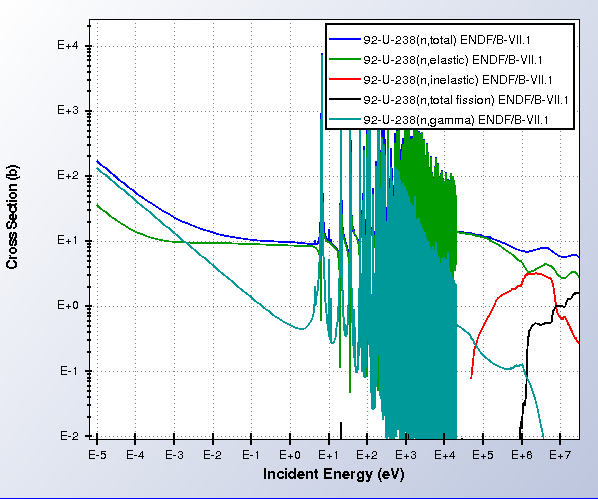
\includegraphics[scale=0.5]{./hw02_08.png}
 % hw02_08.png: 598x499 pixel, 72dpi, 21.10x17.60 cm, bb=0 0 598 499
 \caption{\ce{^{238}U} Neutron Cross sections}
 \label{fig:u238_plot}
\end{figure}

\begin{figure}
 \centering
 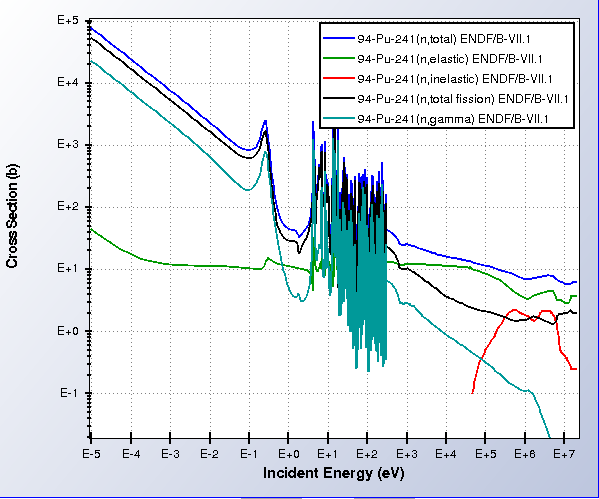
\includegraphics[scale=0.5]{./hw02_08b.png}
 % hw02_08.png: 598x499 pixel, 72dpi, 21.10x17.60 cm, bb=0 0 598 499
 \caption{\ce{^{241}Pu} Neutron Cross sections}
 \label{fig:pu241_plot}
\end{figure}

   

\end{homeworkProblem}




\end{document}
